En este capítulo estudiaremos entonces el problema de enviar símbolos discretos a través de un medio analógico o canal. La Figura \ref{fig:mod_digital_bb} muestra el esquema básico de trabajo. El proceso de entrada es una secuencia de símbolos o proceso estocástico de tiempo discreto, $\{a_k:k\in\mathbb{Z}\}$, que asumiremos WSS y con valores en un alfabeto finito de tamaño $M$.

El sistema debe ser capaz de transmitir dichos símbolos por un canal físico (por ejemplo, par de cobre), utilizando una señal $x(t)$ \emph{que dependa de los símbolos a transmitir} y contenga la información. Dicha señal se verá afectada por el canal (atenuación, limitaciones de ancho de banda, ruido), por lo que la señal $\hat{x}(t)$ no es igual a la señal generada. Sin embargo, si muestreamos la señal en el momento correcto, puede ser posible decodificar el símbolo enviado con baja probabilidad de error.

En este capítulo analizaremos la llamada en \emph{modulación en banda base}, donde la secuencia de símbolos es codificada mediante una sucesión de \emph{pulsos analógicos} que duran un tiempo de símbolo, $T_s$. Como veremos, el pulso rectangular simple no siempre es la mejor opción. La razón por la que se denomina modulación es porque los símbolos digitales \emph{modulan} la secuencia de pulsos. La razón por la que se denomina en banda base es porque no intervienen componentes de alta frecuencia (ver Capítulo \ref{chapter:modulacion pasabanda}).

\begin{figure}[b]
    \begin{center}
        
        \begin{blockdiagram}[node distance=4em]
        \node [block,align=center] (fuente) {Fuente \\ digital};
        \node [block, right = of fuente] (tx) {Transmisor};
        \node [block, right= of tx] (ch) {Canal};
        \node [block, right = of ch] (rx) {Detector};
        \node [block, right = of rx, align=center] (sink) {Receptor \\ digital};

        \draw[thick, ->] (fuente)--node[midway,above] {$a_k$} (tx);
        \draw[thick, ->] (tx)--node[midway,above] {$x(t)$} (ch);
        \draw[thick, ->] (ch)--node[midway,above] {$\hat{x}(t)$} (rx);
        \draw[thick, ->] (rx)--node[midway,above] {$\hat{a}_k$} (sink);
        
        \node [block, below = 2em of ch] (sinc) {Sincronismo};
        \draw[thick, -] (tx) |- (sinc);
        \draw[thick, ->] (sinc) -| (rx);
        \end{blockdiagram}

        \caption{Esquema de un sistema de modulación digital.}\label{fig:mod_digital_bb}
    \end{center}
\end{figure}

Antes de continuar, definamos algunos parámetros relevantes a la hora de cuantificar la transferencia de información.

\begin{definicion}
    Definimos los siguientes parámetros:
    \begin{itemize}
        \item \emph{Velocidad de señalización} $f_s$. Es la frecuencia con la que se envía un símbolo, o bien $f_s=1/T_s$ siendo $T_s$ el tiempo de símbolo. Se mide en $\unit{baudios}:=\rfrac{\text{símbolos}}{\unit{\sec}}$.

    \item \emph{Velocidad de transmisión de información ($\vti$)}. Se mide en bits por segundo o $\unit{\bps}$. Si el alfabeto tiene $M$ símbolos, cada símbolo codifica $\log_2(M)$ bits de información, por lo que:
    \begin{equation*}
        \vti := f_s \log_2(M)
    \end{equation*}
    \item \emph{Ancho de banda del canal $B$} en $\unit{\Hz}$.
    \item \emph{Eficiencia espectral}:
     \begin{equation*}
        \mathrm{Eff} := \frac{\vti}{B},
     \end{equation*}
     y se mide en $\unit{\bps/\Hz}$.
    \end{itemize}
\end{definicion}
La $\vti$ es la velocidad que observa la capa superior. Por ejemplo, el estándar USB 1.1 permite hasta $1.5\unit{\mega\bps}$, mientras que el USB 2.0 lo eleva a $480 \unit{\mega\bps}$. Esa velocidad, como veremos, dependerá del ancho de banda físico $B$, la calidad del canal, así como de las formas de onda que representan los símbolos.

Los problemas que afectan a la transmisión por pulsos se muestran en la Figura \ref{fig:problemas canal}. El resultado final es un pulso distorsionado, pero que adecuadamente muestreado permite recuperar el símbolo transmitido.

\begin{figure}
    \begin{center}
    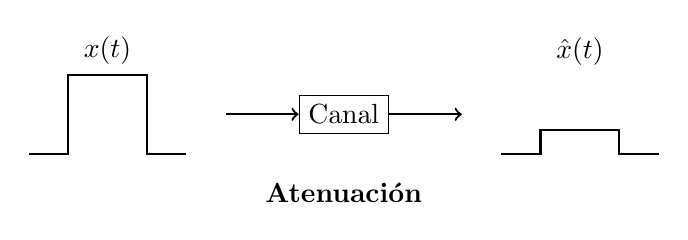
\begin{tikzpicture}
        \draw[thick] (1,0) -- (1.5,0) -- (1.5,1) --node[midway,above] {$x(t)$} (2.5,1) -- (2.5,0) -- (3,0);
        \node[rectangle,draw] at (5,0.5) (canal) {Canal};
        \draw[thick,->] (3.5,.5) -- (canal);
        \draw[thick,->] (canal) -- (6.5,.5);
        \draw[thick] (7,0) -- (7.5,0) -- (7.5,.3) -- (8.5,.3) -- (8.5,0) -- (9,0);
        \node[above] at (8,1) {$\hat{x}(t)$};
        \node at (5,-.5) {\textbf{Atenuación}};
    \end{tikzpicture}\hfill
    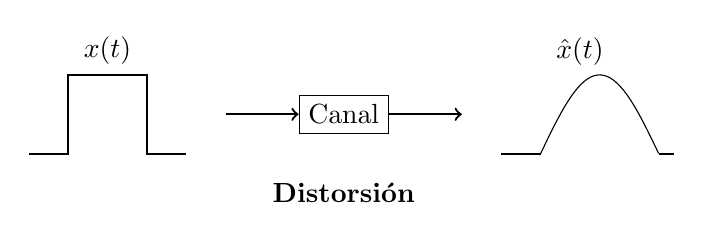
\begin{tikzpicture}
        \draw[thick] (1,0) -- (1.5,0) -- (1.5,1) --node[midway,above] {$x(t)$} (2.5,1) -- (2.5,0) -- (3,0);
        \node[rectangle,draw] at (5,0.5) (canal) {Canal};
        \draw[thick,->] (3.5,.5) -- (canal);
        \draw[thick,->] (canal) -- (6.5,.5);
        \draw[thick] (7,0) -- (7.5,0);
        \draw plot [thick,domain=7.5:9,samples=100] (\x,{sin(2*pi*(\x-7.5)/3 r)});
        \draw[thick] (9,0) -- (9.2,0);
        \node[above] at (8,1) {$\hat{x}(t)$};
        \node at (5,-.5) {\textbf{Distorsión}};
    \end{tikzpicture}
    \bigskip

    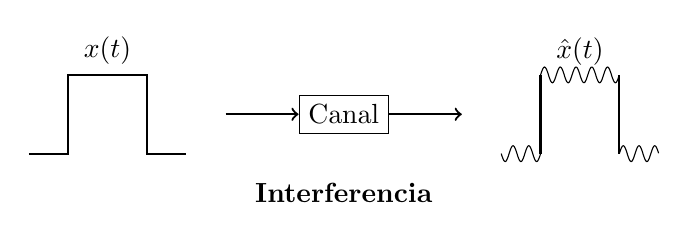
\begin{tikzpicture}
        \draw[thick] (1,0) -- (1.5,0) -- (1.5,1) --node[midway,above] {$x(t)$} (2.5,1) -- (2.5,0) -- (3,0);
        \node[rectangle,draw] at (5,0.5) (canal) {Canal};
        \draw[thick,->] (3.5,.5) -- (canal);
        \draw[thick,->] (canal) -- (6.5,.5);
        \draw plot [thick,domain=7:7.5,samples=100] (\x,{0.1*sin(2*5*pi*(\x-7.5) r)});
        \draw[thick] (7.5,0)--(7.5,1);
        \draw plot [thick,domain=7.5:8.5,samples=100] (\x,{1+0.1*sin(2*5*pi*(\x-7.5) r)});
        \draw plot [thick,domain=8.5:9,samples=100] (\x,{0.1*sin(2*5*pi*(\x-7.5) r)});
        \draw[thick] (8.5,1)--(8.5,0);
        \node[above] at (8,1) {$\hat{x}(t)$};
        \node at (5,-.5) {\textbf{Interferencia}};
    \end{tikzpicture}\hfill
    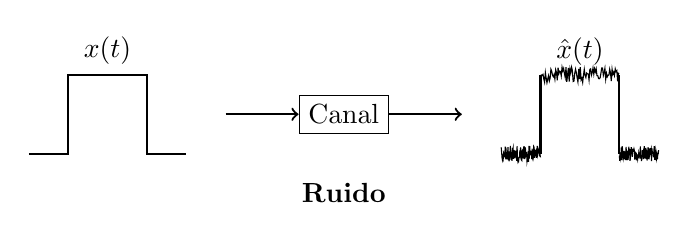
\begin{tikzpicture}
        \draw[thick] (1,0) -- (1.5,0) -- (1.5,1) --node[midway,above] {$x(t)$} (2.5,1) -- (2.5,0) -- (3,0);
        \node[rectangle,draw] at (5,0.5) (canal) {Canal};
        \draw[thick,->] (3.5,.5) -- (canal);
        \draw[thick,->] (canal) -- (6.5,.5);
        \draw plot [thick,domain=7:7.5,samples=100] (\x,.1*rand);
        \draw[thick] (7.5,0)--(7.5,1);
        \draw plot [thick,domain=7.5:8.5,samples=100] (\x,1+.1*rand);
        \draw plot [thick,domain=8.5:9,samples=100] (\x,.1*rand);
        \draw[thick] (8.5,1)--(8.5,0);
        \node[above] at (8,1) {$\hat{x}(t)$};
        \node at (5,-.5) {\textbf{Ruido}};
    \end{tikzpicture}
    \bigskip

    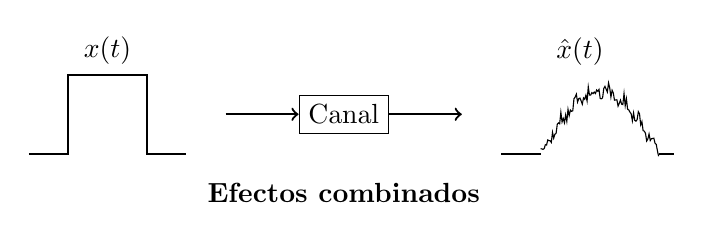
\begin{tikzpicture}
        \draw[thick] (1,0) -- (1.5,0) -- (1.5,1) --node[midway,above] {$x(t)$} (2.5,1) -- (2.5,0) -- (3,0);
        \node[rectangle,draw] at (5,0.5) (canal) {Canal};
        \draw[thick,->] (3.5,.5) -- (canal);
        \draw[thick,->] (canal) -- (6.5,.5);
        \draw[thick] (7,0) -- (7.5,0);
        \draw plot [thick,domain=7.5:9,samples=100] (\x,{0.8*sin(2*pi*(\x-7.5)/3 r)+ .08*rand + 0.05*sin(2*5*pi*(\x-7.5) r)});
        \draw[thick] (9,0) -- (9.2,0);
        \node[above] at (8,1) {$\hat{x}(t)$};
        \node at (5,-.5) {\textbf{Efectos combinados}};
    \end{tikzpicture}



    \caption{Problemas que afectan la transmisión por un canal.}\label{fig:problemas canal}
    \end{center}
\end{figure}

\section{Modulación por pulsos y codificación de línea}

El modelo básico de transmisión de datos en banda base es entonces la \emph{modulación por amplitud de pulsos (pulse amplitude modulation, PAM)}. En este caso, se tiene un proceso de símbolos $\{a_k:k\in\mathbb{Z}\}$ de $M$ símbolos, que interpretaremos como valores por ejemplo de voltaje o amplitud. Luego se eligen:
\begin{itemize}
    \item Un \emph{tiempo de símbolo} $T_s$ que corresponde luego a la frecuencia de señalización $f_s=1/T_s$.
    \item Una forma de pulso $p(t)$ (no necesariamente rectangular).
\end{itemize}

Para lograr la señalización se construye entonces la \emph{onda PAM}:
\begin{equation*}
    x(t) = \sum_{k} a_k p(t-kT_s),
\end{equation*}
es decir, cada símbolo se representa por un pulso de amplitud $a_k$ con origen en el tiempo $kT_s$ para el $k-$ésimo símbolo.

La elección combinada de las amplitudes posibles para $a_k$ y de la forma del pulso $p(t)$ determinan lo que se denomina \emph{codificación de línea}. En la Figura \ref{fig:codlin} se representan algunos códigos de línea utilizados en la práctica.

\begin{figure}
    \begin{center}
        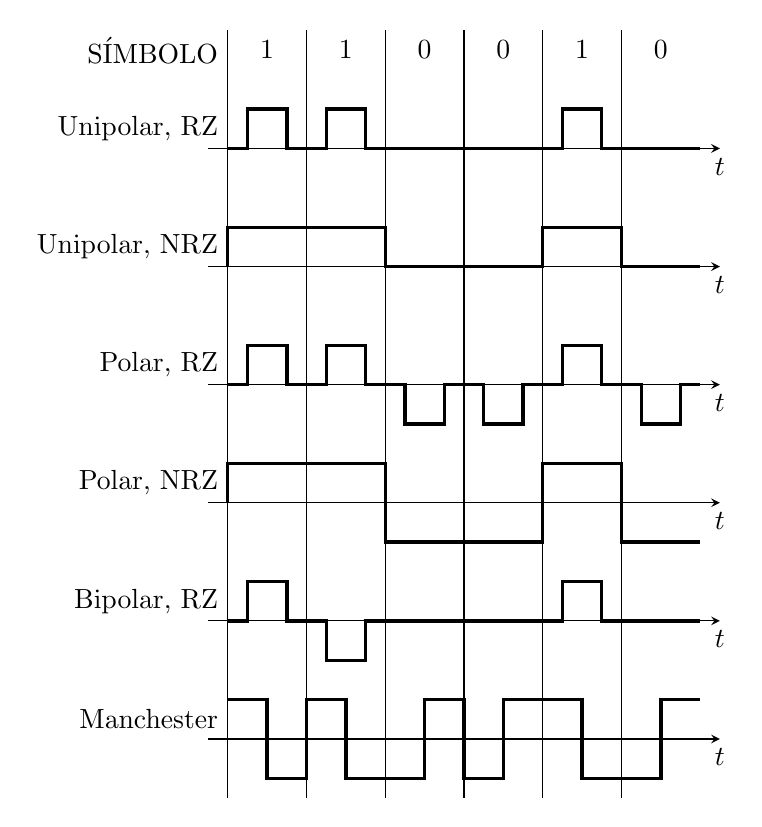
\begin{tikzpicture}[scale=0.5]
            \draw (0,1) -- (0,-18.5);
            \draw (2,1) -- (2,-18.5);
            \draw (4,1) -- (4,-18.5);
            \draw (6,1) -- (6,-18.5);
            \draw (8,1) -- (8,-18.5);
            \draw (10,1) -- (10,-18.5);
            \path (0,0.5) node [anchor=east] {SÍMBOLO} -- (1,0.5) node {$1$} -- (3,0.5) node {$1$} -- (5,0.5) node {$0$} -- (7,0.5) node {$0$} -- (9,0.5) node {$1$} -- (11,0.5) node {$0$};
            \begin{scope}[shift={(0,-2)}]
                \draw[-stealth] (-0.5,0) -- (12.5,0) node [anchor=north] {$t$};
                \path (0,0.5) node [anchor=east] {Unipolar, RZ};
                \draw[very thick] (0,0) -- (0.5,0) -- (0.5,1) -- (1.5,1) -- (1.5,0) -- (2.5,0) -- (2.5,1) -- (3.5,1) -- (3.5,0) -- (8.5,0) -- (8.5,1) -- (9.5,1) -- (9.5,0) -- (12,0);
            \end{scope}
            \begin{scope}[shift={(0,-5)}]
                \draw[-stealth] (-0.5,0) -- (12.5,0) node [anchor=north] {$t$};
                \path (0,0.5) node [anchor=east] {Unipolar, NRZ};
                \draw [very thick] (0,0) -- (0,1) -- (4,1) -- (4,0) -- (8,0) -- (8,1) -- (10,1) -- (10,0) -- (12,0);
            \end{scope}
            \begin{scope}[shift={(0,-8)}]
                \draw[-stealth] (-0.5,0) -- (12.5,0) node [anchor=north] {$t$};
                \path (0,0.5) node [anchor=east] {Polar, RZ};
                \draw [very thick] (0,0) -- (0.5,0) -- (0.5,1) -- (1.5,1) -- (1.5,0) -- (2.5,0) -- (2.5,1) -- (3.5,1) -- (3.5,0) -- (4.5,0) -- (4.5,-1) -- (5.5,-1) -- (5.5,0) -- (6.5,0) -- (6.5,-1) -- (7.5,-1) -- (7.5,0)-- (8.5,0) -- (8.5,1) -- (9.5,1) -- (9.5,0) -- (10.5,0) -- (10.5,-1) -- (11.5,-1) -- (11.5,0) -- (12,0);
            \end{scope}
            \begin{scope}[shift={(0,-11)}]
                \draw[-stealth] (-0.5,0) -- (12.5,0) node [anchor=north] {$t$};
                \path (0,0.5) node [anchor=east] {Polar, NRZ};
                \draw [very thick] (0,0) -- (0,1) -- (4,1) -- (4,-1) -- (8,-1) -- (8,1) -- (10,1) -- (10,-1) -- (12,-1);
            \end{scope}
            \begin{scope}[shift={(0,-14)}]
                \draw[-stealth] (-0.5,0) -- (12.5,0) node [anchor=north] {$t$};
                \path (0,0.5) node [anchor=east] {Bipolar, RZ};
                \draw[very thick] (0,0) -- (0.5,0) -- (0.5,1) -- (1.5,1) -- (1.5,0) -- (2.5,0) -- (2.5,-1) -- (3.5,-1) -- (3.5,0) -- (8.5,0) -- (8.5,1) -- (9.5,1) -- (9.5,0) -- (12,0);
            \end{scope}
            \begin{scope}[shift={(0,-17)}]
                \draw[-stealth] (-0.5,0) -- (12.5,0) node [anchor=north] {$t$};
                \path (0,0.5) node [anchor=east] {Manchester};
                \draw[very thick] (0,1) -- (1,1) -- (1,-1) -- (2,-1) -- (2,1) -- (3,1) -- (3,-1) -- (5,-1) -- (5,1) -- (6,1) -- (6,-1) -- (7,-1) -- (7,1) -- (9,1) -- (9,-1) -- (11,-1) -- (11,1) -- (12,1);
            \end{scope}
        \end{tikzpicture}
        \caption{Ejemplos de códigos de línea para alfabeto binario.}\label{fig:codlin}
    \end{center}
\end{figure}

Algunas definiciones: el código es \emph{unipolar} cuando los símbolos son $a_k\geqslant 0$, es decir, solo amplitudes positivas. Como veremos esto introduce componente de continua, por lo cual a veces es conveniente utilizar una señalización \emph{polar} con símbolos positivos o negativos. También puede ser de interés utilizar codificaciones \emph{bipolares}, donde el mismo símbolo se puede representar alternadamente por valores positivos o negativos, o códigos tipo Manchester, que introducen formas de pulso diferentes para cada símbolo (ver Figura \ref{fig:codlin}).

A su vez, una segunda distinción es entre códigos \emph{sin retorno a cero} o NRZ (non--return--to--zero), en los cuales el voltaje se mantiene durante todo el intervalo, y códigos RZ (return--to-zero), en los cuales el pulso es más corto que el tiempo de símbolo. Veremos ventajas y desventajas de estos mecanismos más adelante. Como segundo ejemplo, en la Figura \ref{fig:linea m-ario} se muestra un ejemplo de codificación \emph{cuaternaria polar} (4 símbolos).

\begin{figure}
    \begin{center}
        \begin{tikzpicture}
            \draw (0,0) -- (0.5,0) -- (0.5,1.5) node [anchor=south east] {$3\,V$} -- (1.5,1.5) -- (1.5,0) -- (2,0);
            \draw (3,0) -- (3.5,0) -- (3.5,0.5) -- (4.5,0.5) node [anchor=south west] {$1\,V$} -- (4.5,0) -- (5,0);
            \draw (6,0) -- (6.5,0) -- (6.5,-0.5) node [anchor=north east] {$-1\,V$} -- (7.5,-0.5) -- (7.5,0) -- (8,0);
            \draw (9,0) -- (9.5,0) -- (9.5,-1.5) node [anchor=north east] {$-3\,V$} -- (10.5,-1.5) -- (10.5,0) -- (11,0);
        \end{tikzpicture}
        \caption{Código cuaternario polar con amplitudes $\pm 1\unit{\volt}$ y $\pm 3\unit{\volt}$}\label{fig:linea m-ario}
    \end{center}
\end{figure}

La codificación de línea elegida determina varias propiedades del sistema:
\begin{itemize}
    \item Contenido de frecuencia de la señal.
    \item Componentes de continua.
    \item Información de sincronismo.
    \item Potencia requerida.
    \item Probabilidad de error de detección en presencia de ruido.
\end{itemize}

Para analizar todo esto, es conveniente tener una representación del \emph{espectro} de esta forma de onda, que será aleatoria. Estudiamos esto a continuación.

\section{Espectro de la onda PAM}

El resultado central es el espectro de la onda PAM aleatoria, dado por el siguiente:
\begin{teorema}[Espectro de la onda PAM]\label{teorema:dep onda pam}
    Sea $\{a_k:k\in\mathbb{Z}\}$ un proceso WSS discreto de símbolos con densidad espectral (discreta) $S_a(\phi)$. Consideremos el proceso estocástico de tiempo continuo:
    \begin{equation}\label{eq:onda pam aleatoria}
        x(t) = \sum_k a_k p(t-kT_s + \theta)
    \end{equation}
    siendo $p(t)$ el pulso de transmisión y $\theta$ una variable aleatoria $\mathrm{Uniforme}[0,T_s]$ e independiente del proceso de símbolos (fase aleatoria). Entonces $x(t)$ es un proceso WSS de tiempo continuo con densidad espectral de potencia:
    \begin{equation}\label{eq:dep onda pam}
    S_x(f) = f_s \left|\hat{P}(f)\right|^2 S_a\left(\frac{f}{f_s}\right),
    \end{equation}
    siendo $\hat{P}(f)$ la transformada de Fourier del pulso $p(t)$.
\end{teorema}

Antes de proceder a la prueba, veamos cómo se conecta con la onda binaria aleatoria analizada en el Ejemplo \ref{ej:onda binaria aleatoria}.
\begin{ejemplo}[Onda binaria aleatoria como onda PAM]

    La onda binaria aleatoria ya estudiada puede considerarse un caso particular de lo anterior, donde:
    \begin{itemize}
        \item $a_k=\pm 1$ independientes y equiprobables. Por lo tanto $\mu=0$ y $\sigma^2=1$, de donde $S_a(\phi) = 1$ constante.
        \item $p(t) = p_{[0,T_s]}(t)$ el pulso rectangular, cuya transformada de Fourier es:
         \begin{equation*}
            p_{[0,T_s]}(t) \fourier T_s \sinc(\pi T_s f) e^{-j\pi T_s f} \Longrightarrow |\hat{P}(f)^2| = T_s^2 \sinc^2(\pi T_s f).
         \end{equation*}
    \end{itemize}
    Utilizando \eqref{eq:dep onda pam} queda:
    \begin{equation*}
        S_x(t) = f_s T_s^2 \sinc^2(\pi T_s f) \sigma^2 = T_s \sinc^2(\pi T_s f),
    \end{equation*}
    es decir, la densidad espectral que ya habíamos calculado.
\end{ejemplo}

\begin{proof}[Prueba del Teorema \ref{teorema:dep onda pam}]
Calculamos la autocorrelación del proceso $y(t)$. Para ello, para un $\theta$ fijo calculamos el valor esperado
condicional $E\left[y(t) y(t+\tau)|\theta\right]$ (sobre el
proceso $\{a_k\}$), y después promediamos en $\theta$ uniforme.
\begin{align*}
    E\left[x(t)x(t+\tau)|\theta\right]  & = \E{\left(\sum_k a_k p(t+\theta-kT_s)\right) \left(\sum_l a_m p(t+\tau+\theta-mT_s)\right)}\\
                        & = \sum_{k,m} \E{a_k a_m} p(t+\theta - kT_s) p(t+\tau+\theta-mT_s)\\
        \underset{\scriptstyle(l=m-k)}{} & =  \sum_{k,l} R_a[l] p(t+\theta-kT_s) p(t+\tau+\theta-lT_s-kT_s)\\
                        & = \sum_l R_a[l] \sum_k p(t+\theta-kT_s)
                        p(t+\tau-lT_s+\theta-kT_s).
\end{align*}

Ahora promedio en $\theta$:
\begin{align}\label{eq.rytau}
    E\left[y(t)y(t+\tau)\right]         & = \frac{1}{T_s}\int_0^{T_s} E\left[y(t)y(t+\tau)|\theta\right]\d\theta  \nonumber \\
                        & = f_s \sum_l R_a(l) \sum_k\int_0^{T_s} p(t+\theta-kT_s) p(t+\theta-kT_s + \tau-lT_s)\d\theta \nonumber\\
\underset{\scriptstyle(\eta=\theta-kT_s+t)}{}    & = f_s  \sum_l R_a(l) \sum_k \int_{t-kT_s}^{t-kT_s+T_s} p(\eta) p(\eta + \tau - lT_s)\d\eta\nonumber\\
                        & = f_s \sum_l R_a(l) \int_{-\infty}^{+\infty} p(\eta) p(\eta + \tau-lT_s)\d\eta\nonumber\\
                        & = f_s \sum_l R_a(l) r_p(\tau-lT_s).
\end{align}

En el último paso introdujimos
\[
r_p(\tau) := \left\langle p(t),p(t+\tau)\right\rangle = \int_{-\infty}^{+\infty} p(t) p(t + \tau)\d t,
\]
autocorrelación del pulso como señal de {\em energía} finita. Notar que el resultado es independiente de $t$.

Un argumento similar (más sencillo) prueba que $E[y(t)]$ es  independiente de $t$. Por lo tanto $y(t)$ es un proceso continuo
estacionario.

Recordamos del curso de Análisis de Se\~nal que la transformada de Fourier de $r_p(\tau)$ es la densidad espectral de energía
$|\hat{P}(f)|^2$. Transformando por Fourier en (\ref{eq.rytau}) obtenemos
\begin{align*}
    S_y(f)  & = f_s \sum_l R_a(l) \e^{-j2\pi(lT_s)f} \overbrace{\mathcal{F}\left[r_p(\tau)\right]}^{\left|\hat{P}(f)\right|^2}\\
        & = f_s \left|\hat{P}(f)\right|^2\sum_l R_a(l) \e^{-j2\pi l
        (\frac{f}{f_s})}.
\end{align*}
Recurriendo a (\ref{eq.safi}) interpretamos la última suma como
$S_a\left(\frac{f}{f_s}\right).$

\end{proof}


\subsection*{Caso particular más usado}

En la Sección \ref{sec.densdig} consideramos un caso particular del proceso de símbolos: $\{a_k\}$ independientes, idénticamente distribuidos, con $E[a_k]=\mu$, $E[a_k^2]=\mu^2+\sigma^2$.
Veamos ahora como particularizar la fórmula (\ref{eq.dig}) a ese caso.

Utilizando la independencia, calculamos la autocorrelación del proceso de símbolos:
\begin{align*}
R_a(l) &= E[a_k a_{k+l}]= \begin{cases}
                                        \mu^2+\sigma^2 & l = 0\\
                                        \mu^2 & l\neq 0
                                       \end{cases} \\
                                       &= \mu^2+\sigma^2\delta(l).
\end{align*}

Su transformada de Fourier de tiempo discreto (función periódica de $\varphi\in\R$) es
\[
  S_a(\varphi) = \sigma^2 + \mu^2 \sum_{n=-\infty}^{+\infty}\delta(\varphi - n).
\]

\[\Rightarrow  S_a\left(\frac{f}{f_s}\right) = \sigma^2+\mu^2\sum_{n=-\infty}^{+\infty} \delta\left(\frac{f-nf_s}{f_s}\right) = \sigma^2+\mu^2 f_s \sum_{n=-\infty}^{+\infty} \delta (f-nf_s).\]

Sustituyendo en (\ref{eq.dig}) llegamos a la fórmula utilizada en la Sección \ref{sec.densdig}.
\begin{equation}
    \label{eq:dig3}
    {\color{Red}\boxed{\normalcolor S_x(f) = \sigma^2 f_s \left|\hat{P}(f)\right|^2 + \mu^2 f_s^2 \sum_{n=-\infty}^{+\infty} \left|\hat{P}(nf_s)\right|^2\delta(f-nf_s)}}\tag{\textasteriskcentered}
\end{equation} 

\section{Formación de pulsos y control del ancho de banda: problema de Nyquist}


\section{Detección sincrónica en presencia de ruido}


\section{Detección óptima: filtro acoplado}


\section{Ecualización de canal}


\section{Repetidores regenerativos}